\section{Auswertung}
\label{sec:Auswertung}
\subsection{Bestimmung der Brennweite aus Gegenstandsweite und Bildweite}
Aus dem Mittelwert der gemessenen Werte wird mithilfe von Gleichung \ref{eqn:linsengl} die Brennweite der Linse bestimmt.
\begin{equation}
    f_1 = \frac{g \cdot b}{g+b} = 95,86 \text{mm} \nonumber
\end{equation}
Die Messung wird nun über das auftragen der Messwerte in einem Koordinatensystem bewertet, wenn die Messgenauigkeit hoch ist, sollten sich alle geraden in einem Punkt schneiden dessen x und y koordinate der Brennwite entsprechen.
\begin{figure}[H]
    \centering
    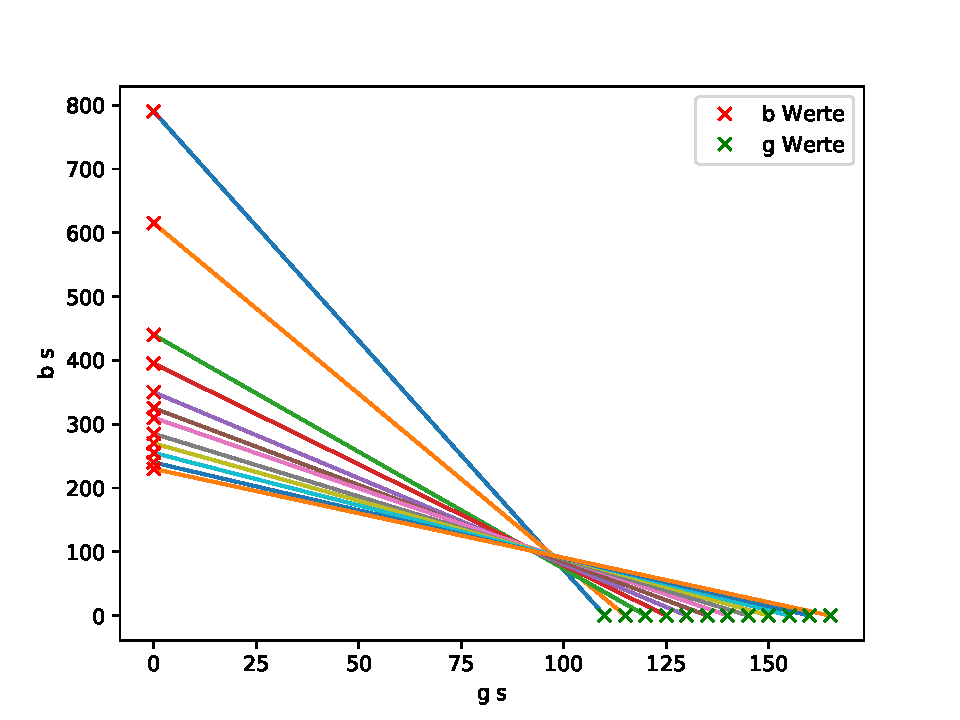
\includegraphics[width=0.6\textwidth]{plots/plot1.pdf}
    \caption{Die Wertepaare werden auf der jeweiligen Achse aufgetragen und durch eine Gerade verbunden}
\end{figure}
Die selbe Methode wird nun auf eine andere Linse mit einer anderen Brennweite angewandt.
Es ergibt sich:
\begin{equation}
    f_2 = 48,07 \text{mm} \nonumber
\end{equation}
Und der entsprachende Graph:
\begin{figure}[H]
    \centering
    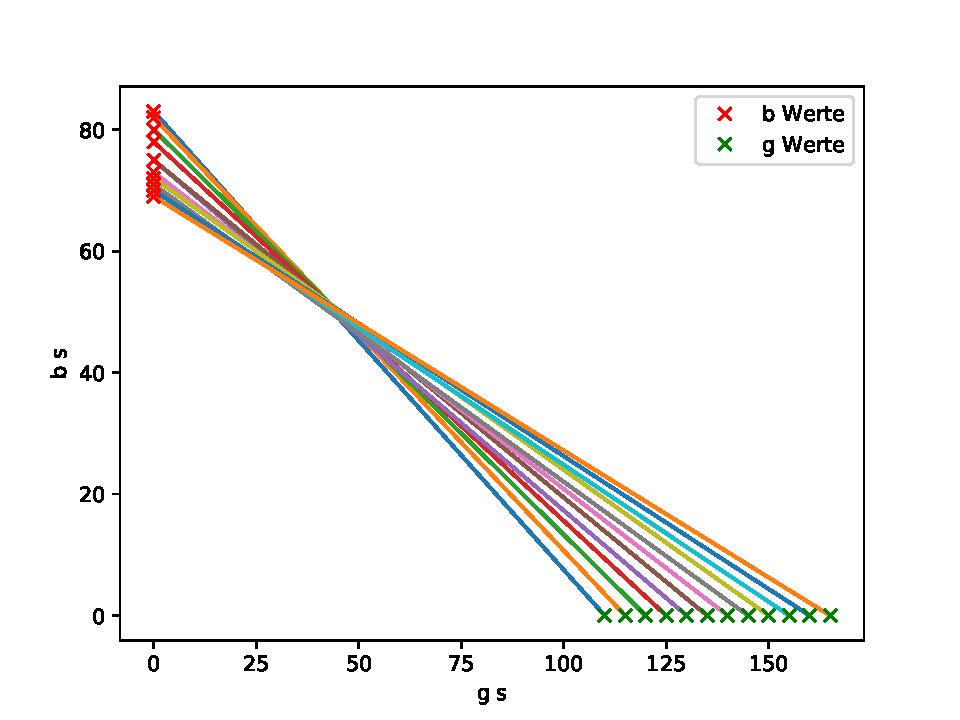
\includegraphics[width=0.6\textwidth]{plots/plot2.pdf}
    \caption{Die Wertepaare werden auf der jeweiligen Achse aufgetragen und durch eine Gerade verbunden}
\end{figure}

\subsection{Methode von Bessel}
Nach der Methode von Bessel lässt sich mit Gleichung \ref{eqn:bessel} die Brennweite der Linse bestimmen.
\begin{table}[H]
    \centering
    \begin{tabular}{c c | c }
        \toprule
        e & d & f\\
        mm & mm & mm\\
        \midrule
        400 & 70 & 96,94\\
        410 & 95 & 97,00\\
        420 & 119& 96,57\\
        430 & 138& 96,43\\
        440 & 155& 96,35\\
        450 & 170& 96,44\\
        460 & 182& 97,00\\
        470 & 193& 97,69\\
        480 & 211& 96,81\\
        490 & 221& 97,58\\
        500 & 233& 97,86 \\
        \bottomrule
    \end{tabular}
    \caption{Die Parameter e und b und die jeweilige berechnete Brennweite}
    \label{tab:tab1}
\end{table}
Als Mittelwert der berechneten Brennweiten ergibt sich
\begin{equation}
    f_{\text{bessel}} = 96,97 \text{mm} \nonumber
\end{equation}
\subsection{Methode von Abbe}
Bei der Methode von Abbe werden die g' und b' aus Gleichung \ref{eqn:abbe1} und \ref{eqn:abbe2} gegen den ensprechenden Term mit V aufgetragen und der lineare Zusammenhang wird untersucht.
\begin{figure}[H]
    \centering
    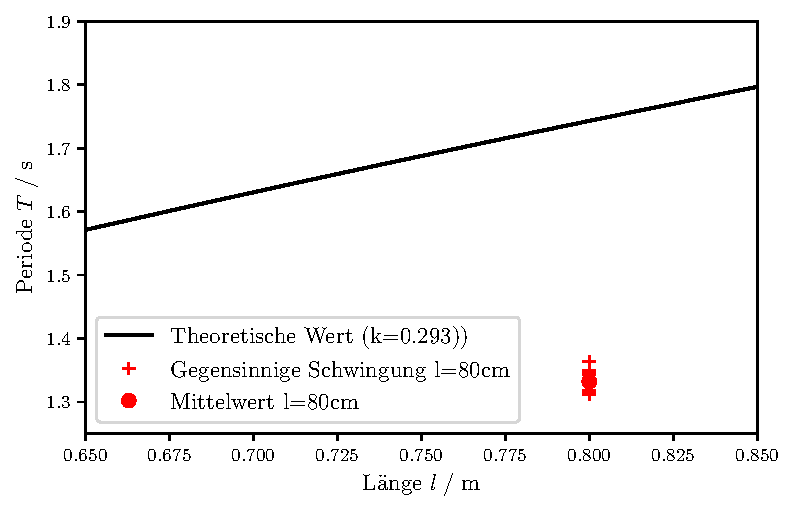
\includegraphics[width=0.6\textwidth]{plots/plot3.pdf}
    \caption{Abbe}
\end{figure}
\begin{figure}[H]
    \centering
    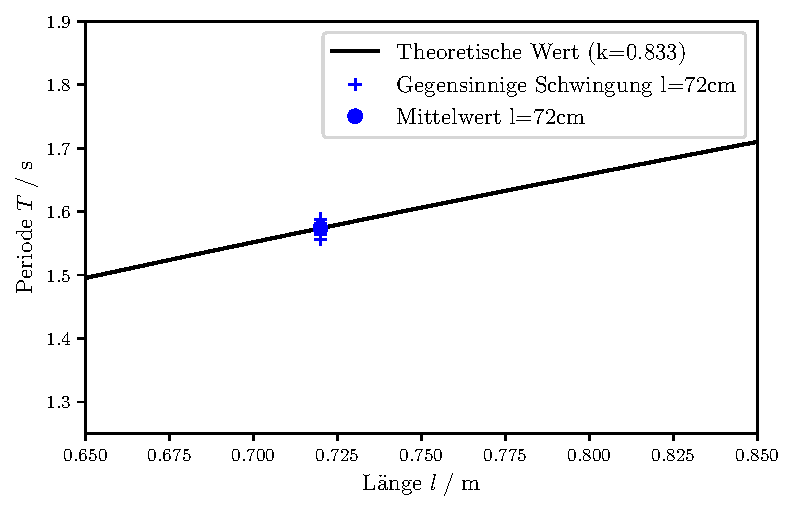
\includegraphics[width=0.6\textwidth]{plots/plot4.pdf}
    \caption{Abbe}
\end{figure}
Bei den hier gemessenen Werten lässt sich nur schwer ein linearer Zusammenhang erkennen.